\vspace{-15pt}
% Comick v3.0 (TheFinalComick)
Plusieurs variantes du réseau pré-entraîné \emph{Resnet18}
\begin{center}

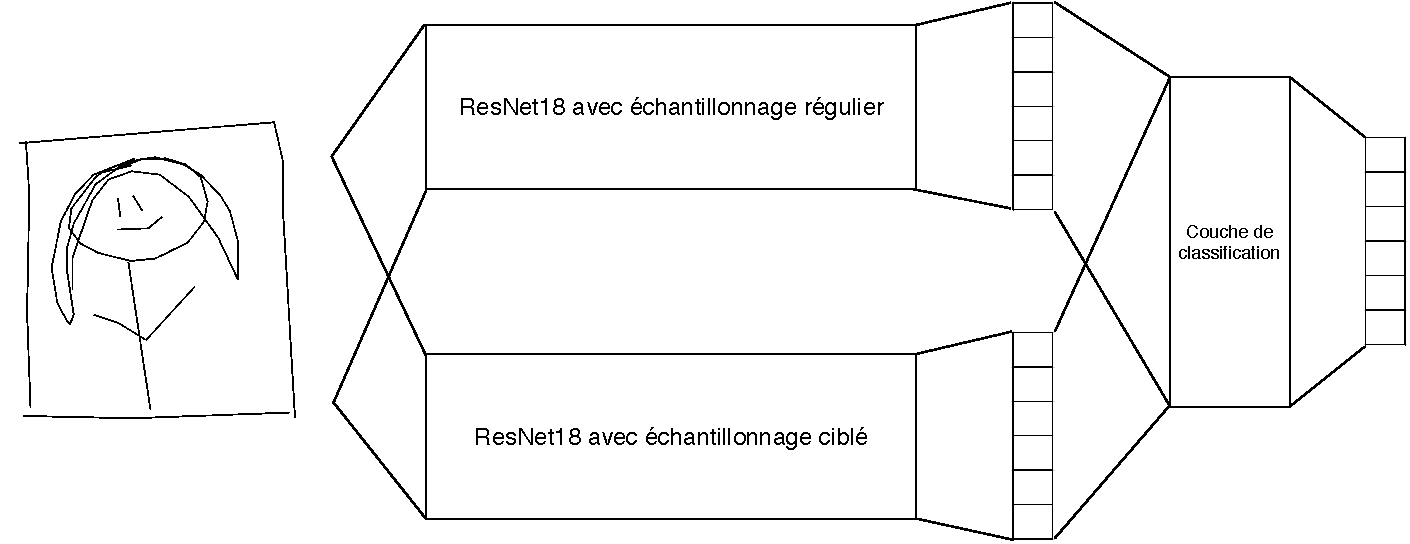
\includegraphics[width=39cm,height=39cm,keepaspectratio]{figures/structure_reseau.pdf}
      
\end{center}

Étant donné les contraintes computationnelles, nous avons utilisé des \emph{epochs} non traditionnelles pour l'entraînement. 
Chaque epoch consiste en un \colorbold{échantillonnage d'un nombre fixe d'images par classe} (ex: 500 images aléatoires par classe; epochs de 170 000 données plutôt que le jeu de données complet).

Similaire à du \colorbold{Bootstrapping} .


\textbf{Variantes:}

\begin{itemize}
\item Échantillonnage variant selon l'exactitude par classe ($\pm$\colorbold{boosting}): $N^*=N(1-accuracy) +0.25N$
\item Méthode par ensemble avec couche de classification
\item Méthode par ensemble avec moyenne
\end{itemize}